\section{Разработка программного средства}
В данном раздела описывается процесс разработки программного \mbox{средства.}

\subsection{Обучение классификатора}
Правильная классификация черт личности является одной из задач данного работы, результат зависит от предподготовки данных, процедуры оценки результата и финального качества обучения.

\begin{figure}[h]
    \centering
    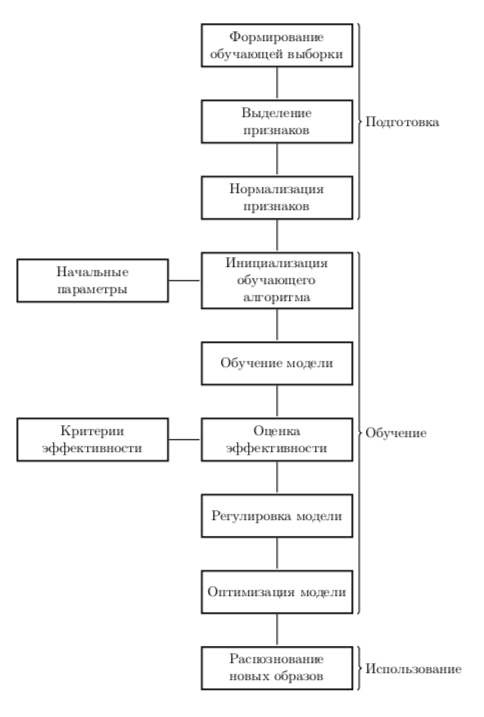
\includegraphics[width=0.7\textwidth]{figures/SVM_flow.png}
    \caption{Алгоритм обучения}
    \label{fig:develoipment:svm_flow}
\end{figure}

Общая схема подготовки, обучения и использования классификатора представлена на рисунке~\ref{fig:develoipment:svm_flow}.

После обучения классификатора можно переходить к классификации образов. 

\subsubsection{Определение характеристик личности}
В листинге~\ref{listing:development:classification} представлен метод классификации нового образца почерка на основе обученной модели. Всего в программном средстве различается 16 типов личности определяющих характеристики.
\begin{figure}[h]
    \centering
    \lstinputlisting[style=commonstyle]{src/evaluate_single_instance.scala}
    \caption{Метод классификации личности по признакам почерка}
    \label{listing:development:classification}
\end{figure}

Для обучения классификатора будет использоваться обучающая выборка <<IAM Handwriting Database>>~\cite{IAM_handwriting_database} состоящая из 1539 образцов текста, написанных 500 авторами, с заранее выделенными признаками почерка либо на основании выделенных параметров можно рассчитать параметры используемые в данной работе. Образцы почерка представлены изображениями в формате png, а параметры XML документом, пример параметров представлен в листинге~\ref{listing:development:sample_set}.
\begin{figure}[h]
    \centering
    \lstinputlisting[style=commonstyle]{src/sample_set.xml}
    \caption{Пример XML-документа описывающего признаки почерка}
    \label{listing:development:sample_set}
\end{figure}

Образцы представлены в выборке в виде png-изображений и для их конвертации в наборы координат используются алгоритмы линейной бинаризации изображений с последующей фильтрацией для удаления шумов и скелетизацией для сокращения объема обрабатываемых данных. Так как ряд динамических параметров, например скорость, не могут быть восстановлены или рассчитаны на основании других параметров они заменяются параметрами по умолчанию. 

Данный объем и содержание обучающей выборки позволяет добиться хорошего качества классификации после обучения благодаря репрезентативности, в частности максимальная разность в количестве образцов разных классов составляет 13\%.

\subsection{Иерархия классов}
\begin{figure}[!ht]
    \centering
    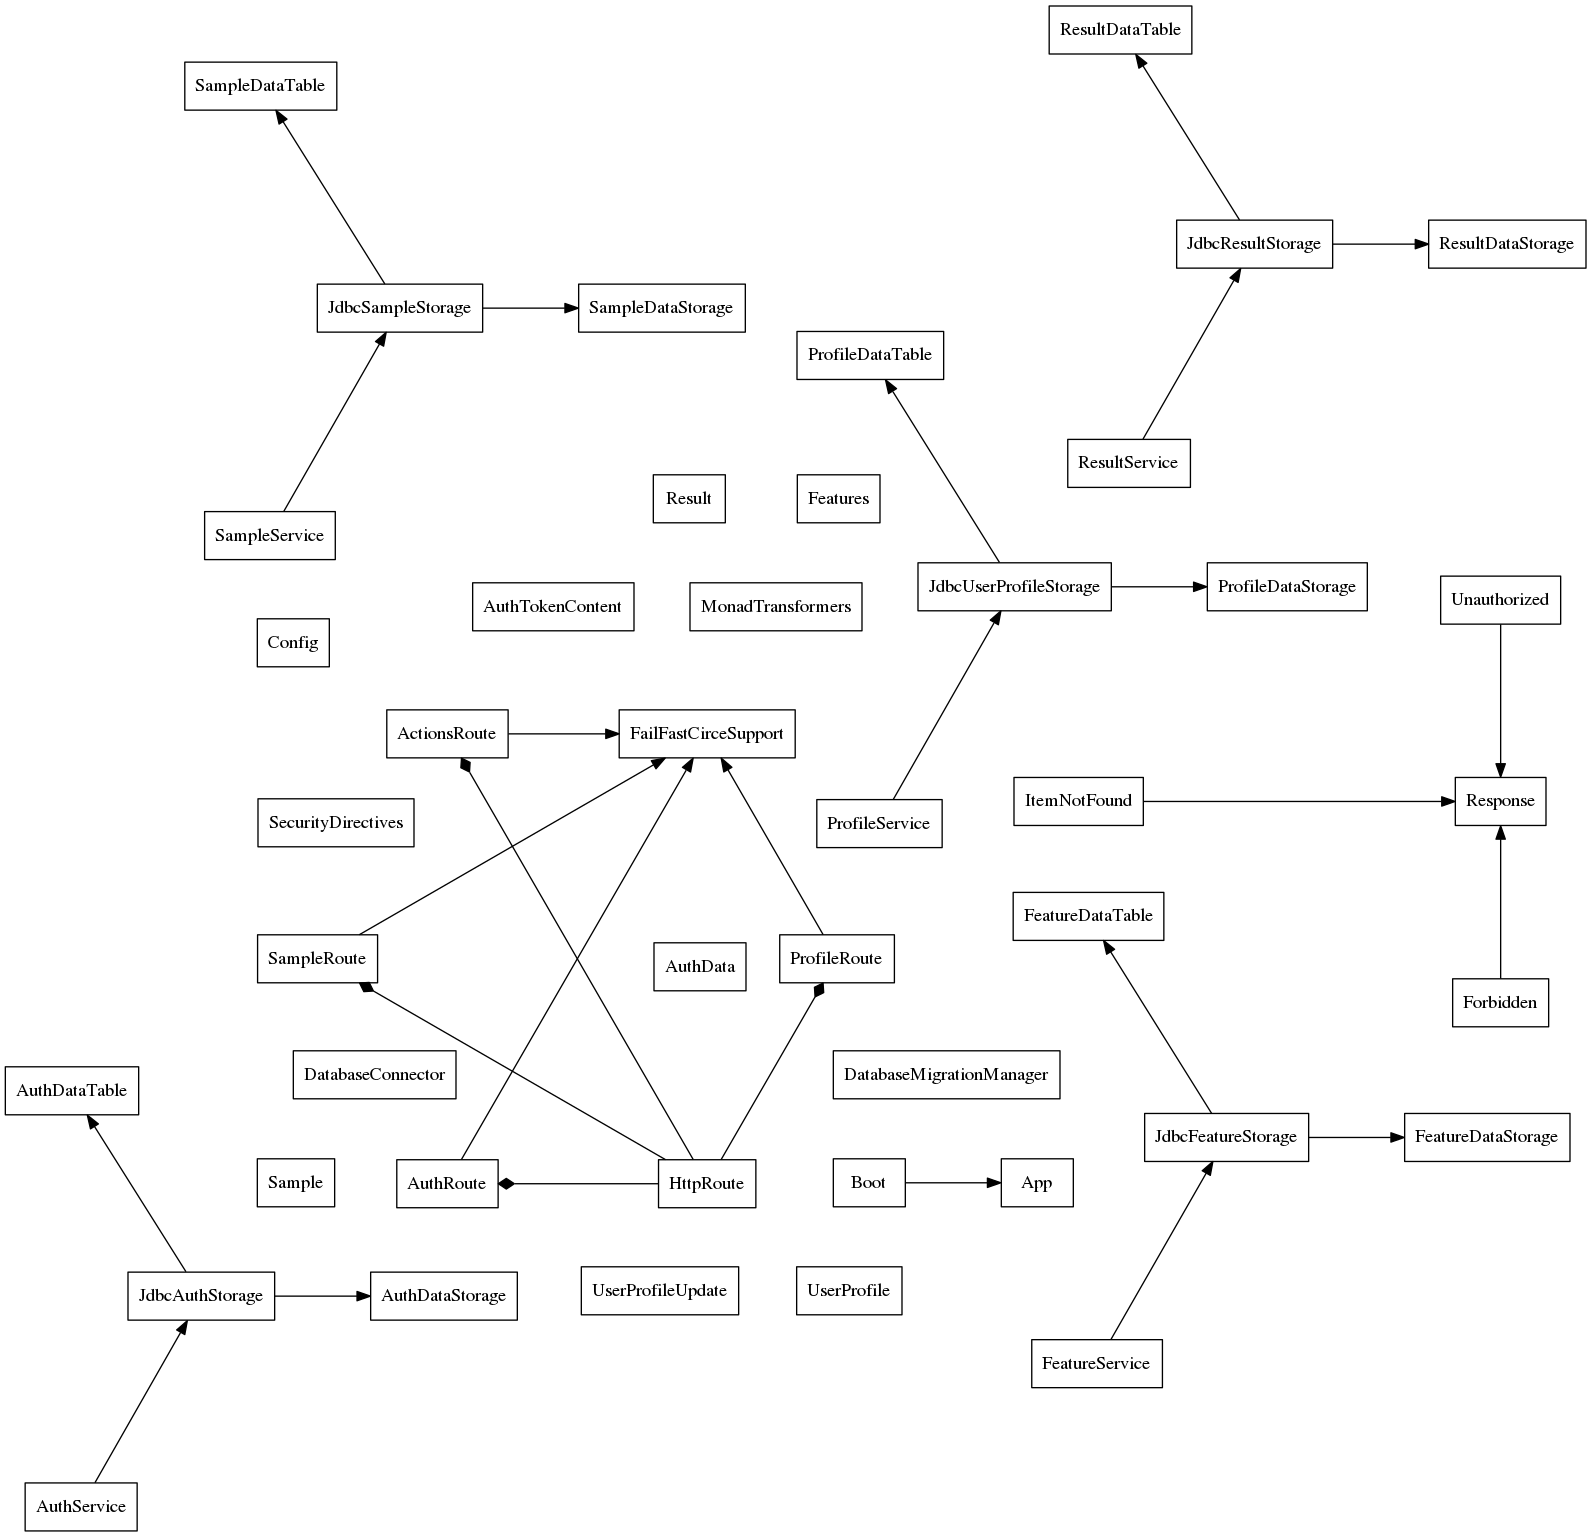
\includegraphics[width=1\textwidth]{figures/classes-fdp.png}
    \caption{Иерархия классов}
    \label{fig:develoipment:class_fdp}
\end{figure}

Общая диаграмма иерархии классов представлена на рисунке~\ref{fig:develoipment:class_fdp}. Все классы отвечающие за обработку запросов и данных, в частности \emph{SampleService}, \emph{ProficeService}, \emph{AuthService} используют контекст исполнения запросов системы акторов библиотеки Akka, описанную в классе \emph{Boot}, благодаря механизму неявных параметров языка Scala. Позволяет обеспечить асинхронную обработку данных и запросов на всех уровнях приложения.

Классы \emph{ItemNotFound}, \emph{Forbidden}, \emph{Unauthorized} являются наследниками класса \emph{Response} и представляют собой обертки для HTTP ответов на различные ошибочные ситуации на стороне клиента.

Классы \emph{Boot}, \emph{App} и \emph{Config} позволяют реализовать механизм управления зависимостями называемый \emph{Cake pattern}. При данном подходе все зависимости модуля, интерфейсы которые он использует в работе, перечисляются в специальной секции. Достоинствами данного подходя является полная поддержка средствами языка и проверка зависимостей на этапе компиляции.

Приведенная диаграмма является обобщенной диаграммой всех модулей и представленные в ней элементы и связи справедливы для всех модулей разработанного программного средства. Различия заключается лишь в функциях классов модуля.

Общая структура разделения кода на классы в каждом модуле позволит упростить понимания взаимодействия классов внутри всех модулей после изучения кода хотя бы одного из них.

\subsection{Маршрутизация запросов}
Библиотека Akka-Http, описанная в пункте~\ref{sec:techs:akka_http}, имеет очень выразительный внутренний язык описания разбора, обработки и маршрутизации запросов к модулю. Модуль доступа к данным является связующий звеном между модулями приложения и базой данных. Поскольку одной из задач программного средства является предотвращение не авторизированного доступа к данным. Каждый обработчик запросов содержит секцию отвечающую за проверку прав доступа.
\begin{figure}[h]
    \centering
    \lstinputlisting[style=commonstyle]{src/routing.scala}
    \caption{Маршрутизация запросов к серверу в модуле доступа к данным}
    \label{listing:development:db_rout}
\end{figure}

Конструкция \emph{authenticate} описанная в классе \emph{SecurityDirectives} отвечает за проверку прав доступа, подробнее будет рассмотрена в разделе~\ref{sec:development:access_control}, а различные функции с префиксом \emph{path} отвечает за маршрутизацию и разбор параметров запросов. 

Использование высоко-интегрированных компонентов, таких как \emph{jwt-scala} позволяет снизить риски некорректной работы при обновлении версий одного из компонентов и ускорить разработку и сопровождения благодаря использованию схожих концепций и стиля разработки.

\subsection{Хранение и передача данных}
Для хранения учетных и пользовательских данных используется СУБД PostgreSQL, схема данных представлена на рисунке~\ref{fig:develoipment:data_base}.

Условно все данные передаваемые между компонентами можно разделить на образцы почерка, листинг~\ref{listing:development:json:sample}, результаты анализа~\ref{listing:development:json:result} и описание пользовательских данных, листинг~\ref{listing:development:json:user}. Для передачи данных между компонентами используется формат JSON с целью, по возможность, исключения или упрощает преобразование информации при общения модулей между собой и с клиентом. 
\begin{figure}[h]
    \centering
    \lstinputlisting[style=commonstyle]{src/sample_result.json}
    \caption{Пример JSON-документа результат анализа на неврологические отклонения}
    \label{listing:development:json:result}
\end{figure}

\begin{figure}[!ht]
    \centering
    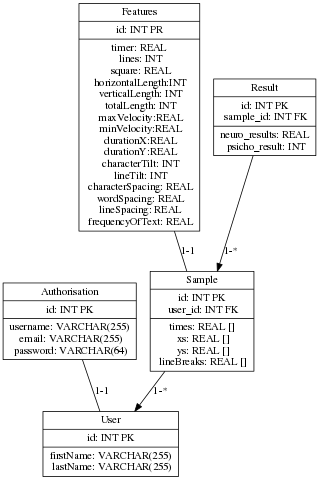
\includegraphics[width=0.7\textwidth]{figures/dataDiagram.png}
    \caption{Схема данных}
    \label{fig:develoipment:data_base}
\end{figure}

\lstinputlisting[
    style=commonstyle,
    caption=Пример JSON-документа описывающего образец текста,
    label=listing:development:json:sample
]{src/sample_item.json}

\lstinputlisting[
    style=commonstyle,
    caption=Пример JSON-документа описывающего пользователя,
    label=listing:development:json:user
]{src/user_item.json}

\subsection{Контроль доступа}
\label{sec:development:access_control}
Для контроля доступа используется механизм основанный на использовании JWT-маркера. Основой данного подхода является использование асинхронной криптографии для подписи и проверки JWT-маркера и доверее информации хранящейся в нем. Для подписи используется алгоритм RSA.

В разрабатываемом программное средстве для обеспечение создания, подписи и проверки JWT-маркеров используется модуль \emph{jwt-scala}. Модуль авторизации после после сравнения имени пользователя и пароля с авторизационных данными хранящимися в базе, создает новый JWT-маркер содержащий уникальный идентификатор пользователя, алгоритм подписи, срок действия, тип маркера, а так же информацию о том является ли он администратором. Далее модуль авторизации подписывает созданный маркер своим секретным ключом и добавляет подпись к маркеру. Так же есть возможность передавать отрытый ключ для его проверки в теле маркера.
Финальное содержание JWT-маркера представлено в листинге~\ref{listing:development:jwt_token}. Далее весь маркер переводится в кодировку Base64, части маркера разделяются точкой, и прикрепляется к ответу клиента.
\lstinputlisting[
    style=commonstyle,
    caption=Пример JWT-маркера,
    label=listing:development:jwt_token
]{src/jwt_token.json}

Клиент получив JWT-маркер использует его для подтверждения прав доступа при запросам к модулям входящим в состав программного средства прикрепляя его к запросам.

Каждый из модулей приложения имеет открытый ключ, являющийся парным к закрытому ключу модуля авторизации, для проверки подлинности подписи маркера. После чего данные содержащиеся в теле маркера могут быть использованы в работе, так как их подлинность доказана. Такой подход позволяет снизить нагрузку на модуль авторизации и базу данных благодаря возможности модуля самостоятельно осуществлять проверку подлинности маркера.

\subsection{Сборка и развертывание}
Для получения последнюю версию исходного кода программного средства используйте команду <<git clone>> в корневом каталоге ПС. Разрешение зависимостей, сборка и развертывание программного средства выполняется с помощью автоматической системы сборки sbt~\cite{sbt}, поэтому перед началом сборки необходимо установить данный инструмент. Программное средство в своей работе использует ряд библиотек. При помощи команды <<sbt>> в корневом каталоге ПС будет произведены загрузка всех необходимых библиотек включая компилятор языка Scala, а так же компиляция модуля программного средства.
Для развертывания модуля программного средства необходимо указать параметры развертывания в файле \emph{application.conf}, подробнее об этом рассказывается в главе~\ref{sec:manpage:admin_man}, и выполнить команду <<sbt run>>. Процесс сборки и развертывания практически полностью выполняется автоматически и не должен вызвать проблем.

Помимо этого сборка и развертывание приложения на тестовом окружении осуществляется автоматически при внесении изменений в базу исходного кода командой <<git push>>.

В данном разделе была рассмотрена общая структура обучение классификатора на основе метода опорных векторов, диаграмма иерархии классов разработанного программного средства, формата хранения данных внутри приложения, таких как учетные записи пользователей и образцы почерка, а так же внешние данные, обучающую выборку. На данном этапе разработка и отладка программное средства закончена и можно переходи к его тестированию.

\subsection{Тестирование программного средства}
\label{sec:testing}
Разработанное программное средство представляет собой набор программных модулей и сервер базы данных. Тестирование программного средства представляет собой проверку работоспособности самих разработанных модулей независимо от сервера базы данных. 
Перед подготовкой программного средства к тестированию необходимо выполнить следующие действия:
\begin{enumerate}
  \item сконфигурировать доступ к базе данных;
  \item сконфигурировать адрес веб-сервера;
  \item развернуть программное средство.
\end{enumerate}

Для оценки правильности работы программного средства было проведено тестирование.

\subsection{Методика использования программного средства}
\label{sec:manpage:admin_man}
Программное средство анализа почерка на основе траектории линий в психологии, медицине и информационной безопасности работает как веб-приложение. Ниже приведено описание вариантов использования и конфигурации модулей приложения.

\subsubsection{Документация Swagger}
Каждый модуль имеет самостоятельную документацию реализованную с помощью инструмента Swagger.
Данная документации содержит следующую информацию:
\begin{itemize}
    \item типы доступных запросов;
    \item коды возможных ответов;
    \item типы и обязательность параметров;
    \item параметры ответа.
\end{itemize}

Просмотреть документацию можно с помощью запроса \mbox{\emph{URL"=модуля/docs}}

\subsubsection{Конфигурация модулей}
Конфигурация модулей осуществятся с помощью файла \emph{application.conf} расположенного в папке \emph{resources} в каталоге с файлами модуля. Для описания конфигурации используется формат HOCON позволяющий представить конфигурацию в легко-читаемом форме. 

\lstinputlisting[
    style=commonstyle,
    caption=Пример файла конфигурации модуля,
    label=listing:manpage:admin_man:app_conf
]{src/application.conf}

Варьируя параметры \emph{host} и \emph{port} можно добиться развертывания модуля на произвольном адресе.

\subsubsection{Конфигурация подключения к БД}
Помимо параметров развертывания и адресов других модулей файл конфигурации модуля доступа к данным содержит блок отвечающий за информацию о базе данных.

\lstinputlisting[
    style=commonstyle,
    caption=Пример блока конфигурации доступа к базе данных,
    label=listing:manpage:admin_man:db_conf
]{src/postgresql.conf}

Наиболее важными параметрами являются \emph{jdbc-url}, \emph{username} и \emph{password}. С помощью параметра \emph{jdbc-url} указывается адрес сервера баз данных и имя базы, а параметра \emph{username} и \emph{password} отвечают за данные для авторизации. Так же при низкой скорость интернет соединения может возникнуть необходимость увеличить значение параметра \emph{connection-timeout}.